% Rapport DevOps - Goat Calendar
\documentclass[a4paper,11pt]{article}

\usepackage[utf8]{inputenc}
\usepackage[T1]{fontenc}
\usepackage[french]{babel}
\usepackage[a4paper,margin=2.3cm]{geometry}
\usepackage{graphicx}
\usepackage{xcolor}
\usepackage{hyperref}
\usepackage{longtable}
\usepackage{booktabs}
\usepackage{array}
\usepackage{enumitem}
\usepackage{listings}
\usepackage{caption}
\usepackage{float}
\usepackage{needspace}
\usepackage{placeins}
\usepackage{etoolbox}

\hypersetup{
  colorlinks=true,
  linkcolor=black,
  urlcolor=blue,
  citecolor=black
}

\definecolor{codebg}{RGB}{248,248,248}
\definecolor{codeborder}{RGB}{210,210,210}
\definecolor{darkblue}{RGB}{20,55,100}

\lstdefinelanguage{Mermaid}{
  morekeywords={flowchart,graph,sequenceDiagram,participant,container,subgraph,end,classDiagram,class,erDiagram,theme,themeVariables,init},
  sensitive=true,
  morecomment=[l]{\%\%}
}

\lstset{
  basicstyle=\ttfamily\small,
  breaklines=true,
  frame=single,
  rulecolor=\color{codeborder},
  backgroundcolor=\color{codebg},
  keywordstyle=\color{darkblue}\bfseries,
  showstringspaces=false,
  columns=fullflexible,
  keepspaces=true
}
\sloppy
\pretocmd{\section}{\FloatBarrier\Needspace{12\baselineskip}}{}{}
\pretocmd{\subsection}{\Needspace{8\baselineskip}}{}{}

\newcommand{\topasset}[2]{%
  \begin{minipage}{0.3\linewidth}
    \centering
    \includegraphics[height=1.9cm,keepaspectratio]{#1}\\
    {\small #2}
  \end{minipage}
}

\title{\textbf{Rapport de projet DevOps}\\Goat Calendar}
\author{Antonin Durand \and Yann Renvoisé}
\date{Juin 2026}

\begin{document}

\pagenumbering{gobble}
\begin{titlepage}
  \centering
  \vspace*{1cm}
  
\includegraphics[height=2.4cm,keepaspectratio]{assets/logo_efrei.png}

  \vspace{2cm}
  {\Large Rapport de projet DevOps\par}
  \vspace{0.6cm}
  {\Huge\bfseries Goat Calendar\par}

  \vspace{1.2cm}
  {\large Application de gestion de boards collaboratifs\par}
  \vspace{0.4cm}
  {\large Backend FastAPI, front web statique, MySQL et Docker Compose\par}

  \vfill
  \begin{tabular}{rl}
    \textbf{Étudiants :} & Antonin Durand \\
                         & Yann Renvoisé \\
    \textbf{Classe :} & Ingé2 LSI2 \\
    \textbf{Année :} & 2025--2026 \\
    \textbf{Date :} & Juin 2026 \\
  \end{tabular}

  \vfill
  \textbf{Lien du dépôt Git :}\\
  \href{https://github.com/GoatsSoftware/GoatCalendar}{https://github.com/GoatsSoftware/GoatCalendar}
\end{titlepage}

\pagenumbering{roman}
\tableofcontents
\newpage
\pagenumbering{arabic}

\section{Introduction}

Goat Calendar est un projet DevOps réalisé en binôme. L'application permet de se connecter, consulter les boards disponibles, créer ou modifier des boards, afficher le détail d'un board, gérer ses rows, tasks, columns, comments, events et permissions.

Le sujet impose un dépôt Git, une pipeline CI, une architecture logicielle en couches, au moins deux services backend intégrés avec Docker, des tests par couche, une couverture de code et une qualité logicielle élevée. La base de données et le front web sont notés en bonus. Dans la version analysée, le projet contient trois services backend, un front web statique, une base MySQL, une orchestration Docker Compose, des tests Pytest, Ruff et une configuration SonarCloud.

\section{Synthèse des exigences}

\begin{longtable}{p{0.35\linewidth}p{0.55\linewidth}}
\toprule
\textbf{Exigence} & \textbf{État dans Goat Calendar} \\
\midrule
Dépôt Git & Le rapport garde le lien du dépôt officiel. \\
Pipeline CI & Lance l'analyse SonarCloud, éxécute les tests unitaires, d'intégratio net de bout-en-bout, et publie dans PyPI les services Python et les images dans DockerHub.  \\
Architecture en couches & Présente : routes FastAPI, services métier, repositories SQLModel, schémas et DTO partagés. \\
Au moins deux services back & Présente : auth\_service, board\_service et database\_service. \\
Intégration Docker & Présente : Docker Compose, trois images backend et un conteneur front Nginx. \\
Tests unitaires et mocks web & Présente : 93 fonctions de test Pytest réparties dans les packages backend. \\
Couverture de code & Sonar attend quatre rapports XML dans \texttt{coverage-reports}. Les fichiers de rapport ne sont pas versionnés dans la copie locale. \\
Qualité logicielle & Ruff configuré dans les packages Python et SonarCloud configuré à la racine. \\
Front web bonus & Présente : HTML, CSS et JavaScript natif servis par Nginx sur le port 8080. \\
Base de données bonus & Présente : MySQL 9.6.0, SQLModel, aiomysql, seed automatique. \\
Google Labs & Emplacements réservés pour les captures d'écran démontrant la complétion des labs. \\
\bottomrule
\end{longtable}

\section{Architecture générale}

Le projet est organisé autour de quatre blocs applicatifs :

\begin{itemize}[leftmargin=*]
  \item \textbf{front\_service} : interface web statique servie par Nginx, pages login, dashboard et détail de board.
  \item \textbf{auth\_service} : authentification OAuth2 password flow, émission et vérification de tokens JWT, gestion des utilisateurs.
  \item \textbf{board\_service} : API principale des boards, colonnes, lignes, tâches, commentaires, événements et permissions.
  \item \textbf{database\_service} : fournit le connecteur à la base de données, la création des tables à partir des schémas SQLModel et le seeding d'un jeu de données de base.
  \item \textbf{shared\_models} : schémas SQLModel, DTO, enums, settings, exceptions et types communs aux services backend.
\end{itemize}

\subsection{Schéma d'architecture}

\begin{figure}[H]
  \centering
  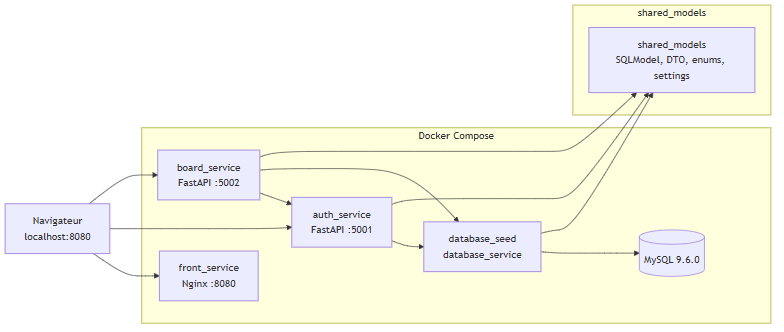
\includegraphics[width=\linewidth,height=0.72\textheight,keepaspectratio]{assets/diagrams/architecture.png}
  \caption{Architecture applicative générée depuis Mermaid}
\end{figure}

\section{Front web}

Le front est volontairement simple et sans framework JavaScript. Il est composé de pages HTML, de CSS par responsabilité et de modules JavaScript natifs. En développement, il peut être servi avec \texttt{py -m http.server 8080}. En production Docker, il est copié dans \texttt{/usr/share/nginx/html} et servi par \texttt{nginx:1.27-alpine}.

Les URLs des API sont centralisées dans \texttt{front/scripts/config.js} :

\begin{itemize}[leftmargin=*]
  \item Auth service : \texttt{http://localhost:5001}
  \item Board service : \texttt{http://localhost:5002}
\end{itemize}

\subsection{Pages principales}

\begin{itemize}[leftmargin=*]
  \item \textbf{Login page} : page \texttt{front/index.html}, formulaire email/password, boutons de comptes démo, récupération et stockage des tokens.
  \item \textbf{Dashboard page} : page \texttt{front/dashboard.html}, liste des boards, création de board, recherche utilisateurs, profil utilisateur.
  \item \textbf{Board page} : page \texttt{front/board.html}, chargement d'un board, affichage des rows et tasks, gestion columns, events et permissions.
\end{itemize}

\subsection{Captures front de démonstration (3 pages)}

\begin{figure}[H]
  \centering
  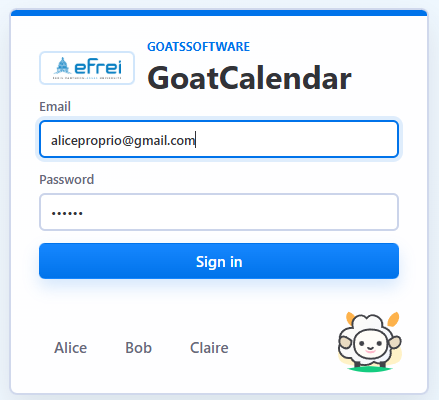
\includegraphics[width=0.85\linewidth]{assets/login_page.png}
  \caption{Login page de Goat Calendar}
\end{figure}

\begin{figure}[H]
  \centering
  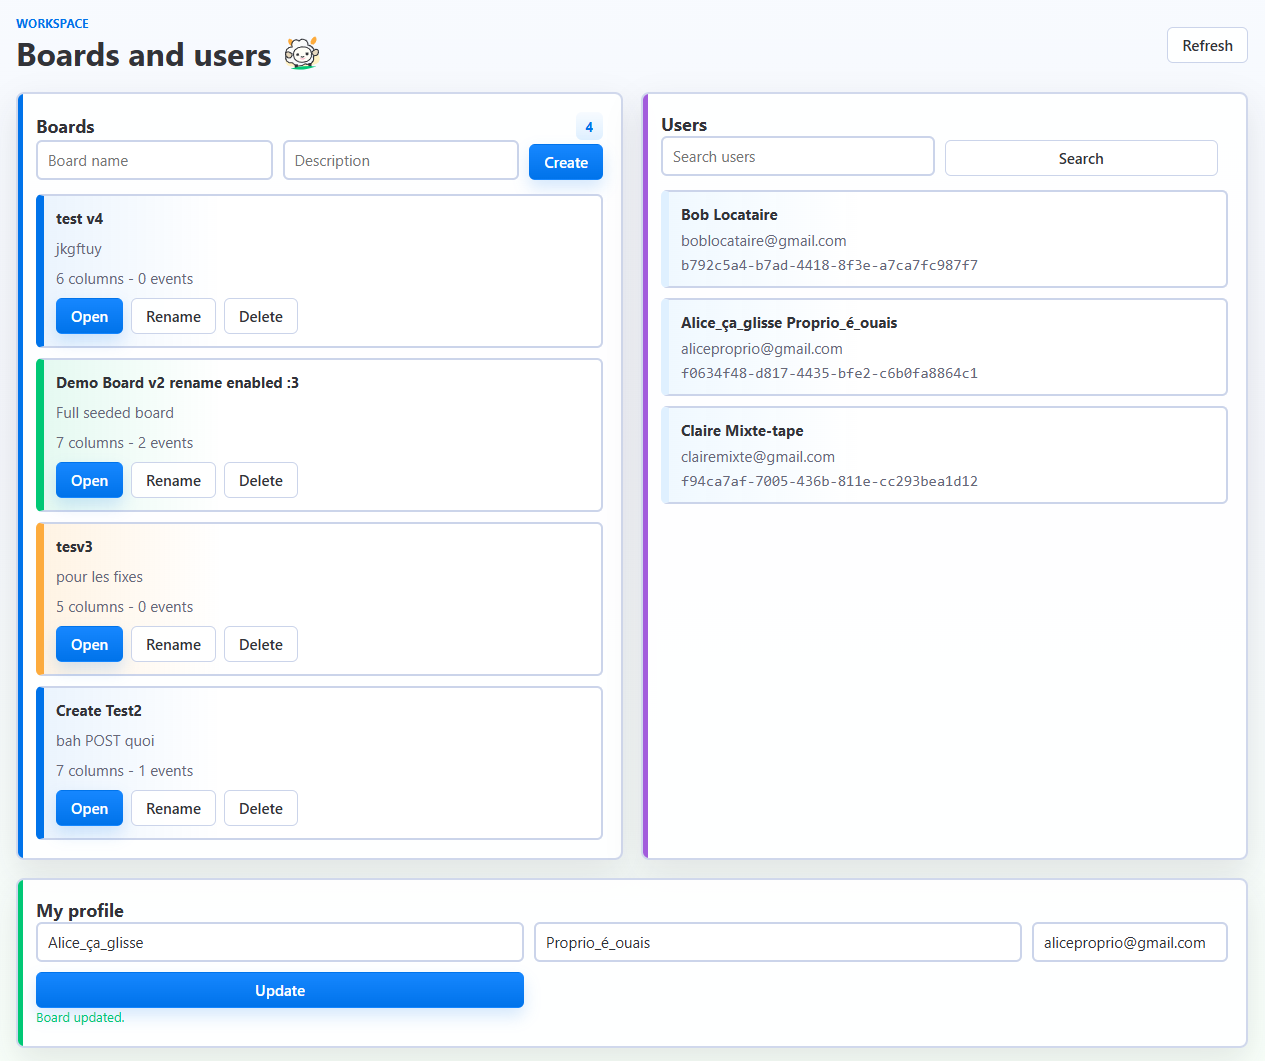
\includegraphics[width=0.85\linewidth]{assets/dashboard_page.png}
  \caption{Dashboard page avec boards, utilisateurs et profil}
\end{figure}

\begin{figure}[H]
  \centering
  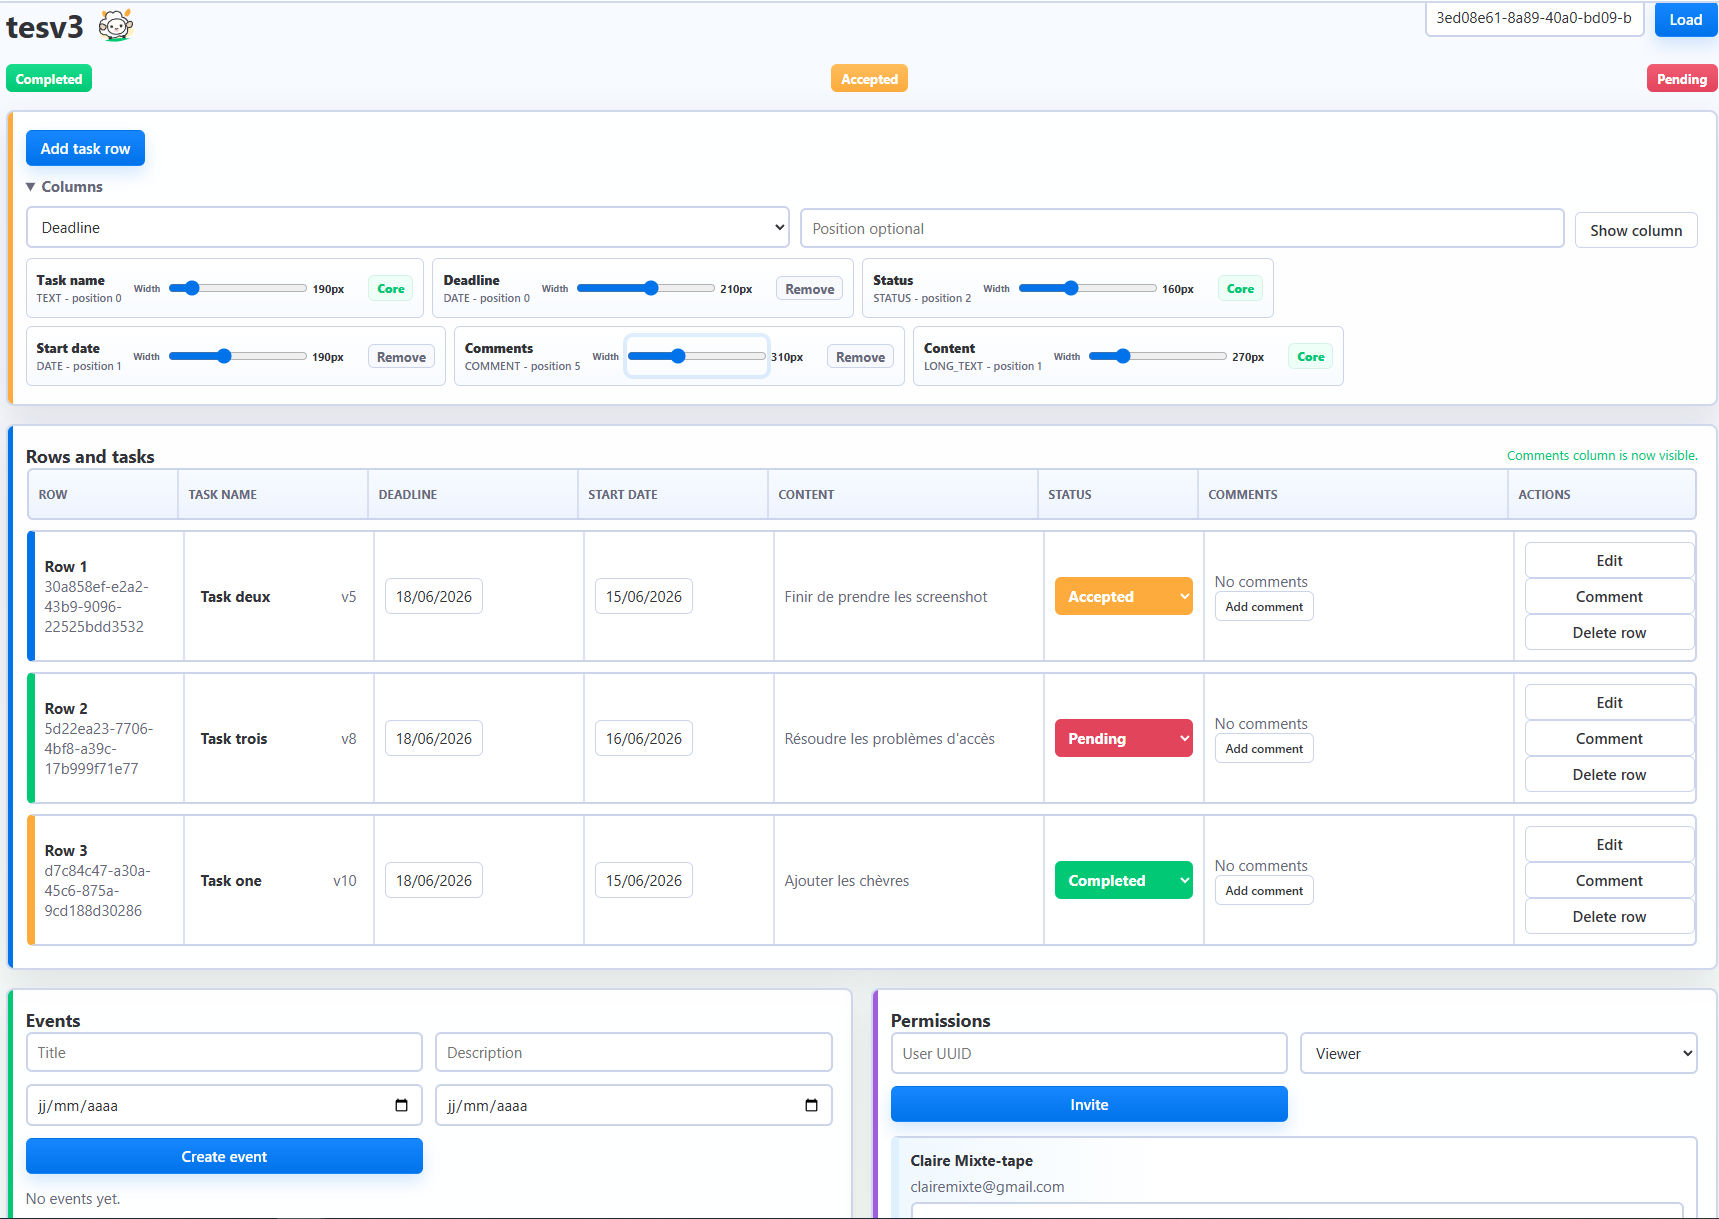
\includegraphics[width=0.85\linewidth]{assets/board_page.png}
  \caption{Board page avec détail des rows d'un board}
\end{figure}

\section{Architecture en couches}

Les services backend suivent une architecture en couches conforme au sujet :

\begin{itemize}[leftmargin=*]
  \item \textbf{Controller/Web} : fichiers \texttt{routes/*.py}. Ils exposent les endpoints FastAPI, injectent les dépendances et convertissent les erreurs en réponses HTTP.
  \item \textbf{Services} : fichiers \texttt{services/*.py}. Ils portent la logique métier, la sérialisation DTO et les règles de création/mise à jour.
  \item \textbf{Data/Repositories} : fichiers \texttt{repositories/*.py} et \texttt{database.py}. Ils exécutent les requêtes SQLModel/SQLAlchemy.
  \item \textbf{Shared models} : fichiers \texttt{shared\_models/*.py}. Il centralise tables, DTO, enums, settings et exceptions.
\end{itemize}

\begin{figure}[H]
  \centering
  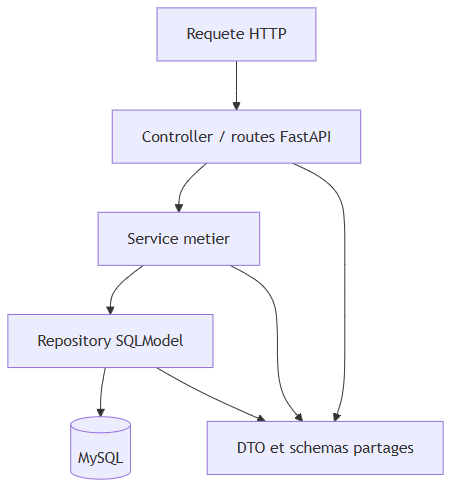
\includegraphics[width=0.86\linewidth,height=0.6\textheight,keepaspectratio]{assets/diagrams/layers.png}
  \caption{Architecture en couches générée depuis Mermaid}
\end{figure}

\section{Description des services backend}

\subsection{\texorpdfstring{\texttt{auth\_service}}{auth service}}

Le service d'authentification est une application FastAPI exposée sur le port 5001. Il utilise une base MySQL via SQLModel et le package \texttt{database\_service} pour obtenir les sessions de base de données.

Routes principales :

\begin{itemize}[leftmargin=*]
  \item \texttt{POST /authentication/auth} : authentifie un utilisateur et retourne une paire de tokens JWT.
  \item \texttt{POST /authentication/refresh\_access\_token} : régénère un token d'accès à partir d'un refresh token.
  \item \texttt{GET /authentication/me} : retourne l'utilisateur connecté.
  \item \texttt{GET /users}, \texttt{GET /users/me}, \texttt{GET /users/search}, \texttt{PUT /users/me} : consultation et modification des utilisateurs.
  \item \texttt{GET /auth\_monitoring/health} : healthcheck du service.
\end{itemize}

La sécurité repose sur OAuth2PasswordBearer, des mots de passe hashés avec Argon2 via Passlib, et des tokens signés avec \texttt{python-jose}. Les durées de token sont configurées par variables d'environnement.

\subsection{\texorpdfstring{\texttt{board\_service}}{board service}}

Le service Board est une application FastAPI exposée sur le port 5002. Il dépend de l'auth\_service pour récupérer l'utilisateur courant via la dépendance \texttt{get\_current\_user}. Il gère le domaine principal de l'application.

Routes principales :

\begin{itemize}[leftmargin=*]
  \item \texttt{/boards} : CRUD des boards et recherche des boards d'un utilisateur.
  \item \texttt{/board\_columns} : colonnes fonctionnelles d'un board.
  \item \texttt{/board\_rows} : lignes horizontales d'un board.
  \item \texttt{/board\_row\_tasks} : tâches rattachées à une ligne et à une colonne.
  \item \texttt{/board\_row\_comments} : commentaires rattachés à une ligne.
  \item \texttt{/board\_events} : événements et jalons d'un board.
  \item \texttt{/boards/\{board\_id\}/permissions} : rôles utilisateurs sur un board.
  \item \texttt{/board\_monitoring/health} : healthcheck du service.
\end{itemize}

\subsection{\texorpdfstring{\texttt{database\_service}}{database service}}

Le service \texttt{database\_service} fournit le connecteur à la base de données, la création des tables à partir des schémas SQLModel et le seeding d'un jeu de données de base. Dans Docker Compose, il est exécuté comme un conteneur court nommé \texttt{database\_seed}. Son script principal lance \texttt{create\_db\_and\_tables()}, puis \texttt{base\_seeder()}.

La connexion utilise SQLModel, SQLAlchemy async engine et aiomysql. Une stratégie de retry attend la disponibilité de MySQL avec 10 tentatives espacées de 5 secondes.

\subsection{\texorpdfstring{\texttt{shared\_models}}{shared models}}

Ce package contient les entités de domaine et les objets d'échange :

\begin{itemize}[leftmargin=*]
  \item tables : \texttt{User}, \texttt{Board}, \texttt{BoardColumn}, \texttt{BoardRow}, \texttt{BoardRowTask}, \texttt{BoardRowComment}, \texttt{BoardEvent}, \texttt{UserBoardPermission} ;
  \item DTO d'entrée et de sortie pour les endpoints ;
  \item enums : rôles, statuts, types de colonnes, type de token, statut de santé ;
  \item settings : configuration serveur, base de données et authentification.
\end{itemize}

\section{Modèle de données}

\begin{figure}[H]
  \centering
  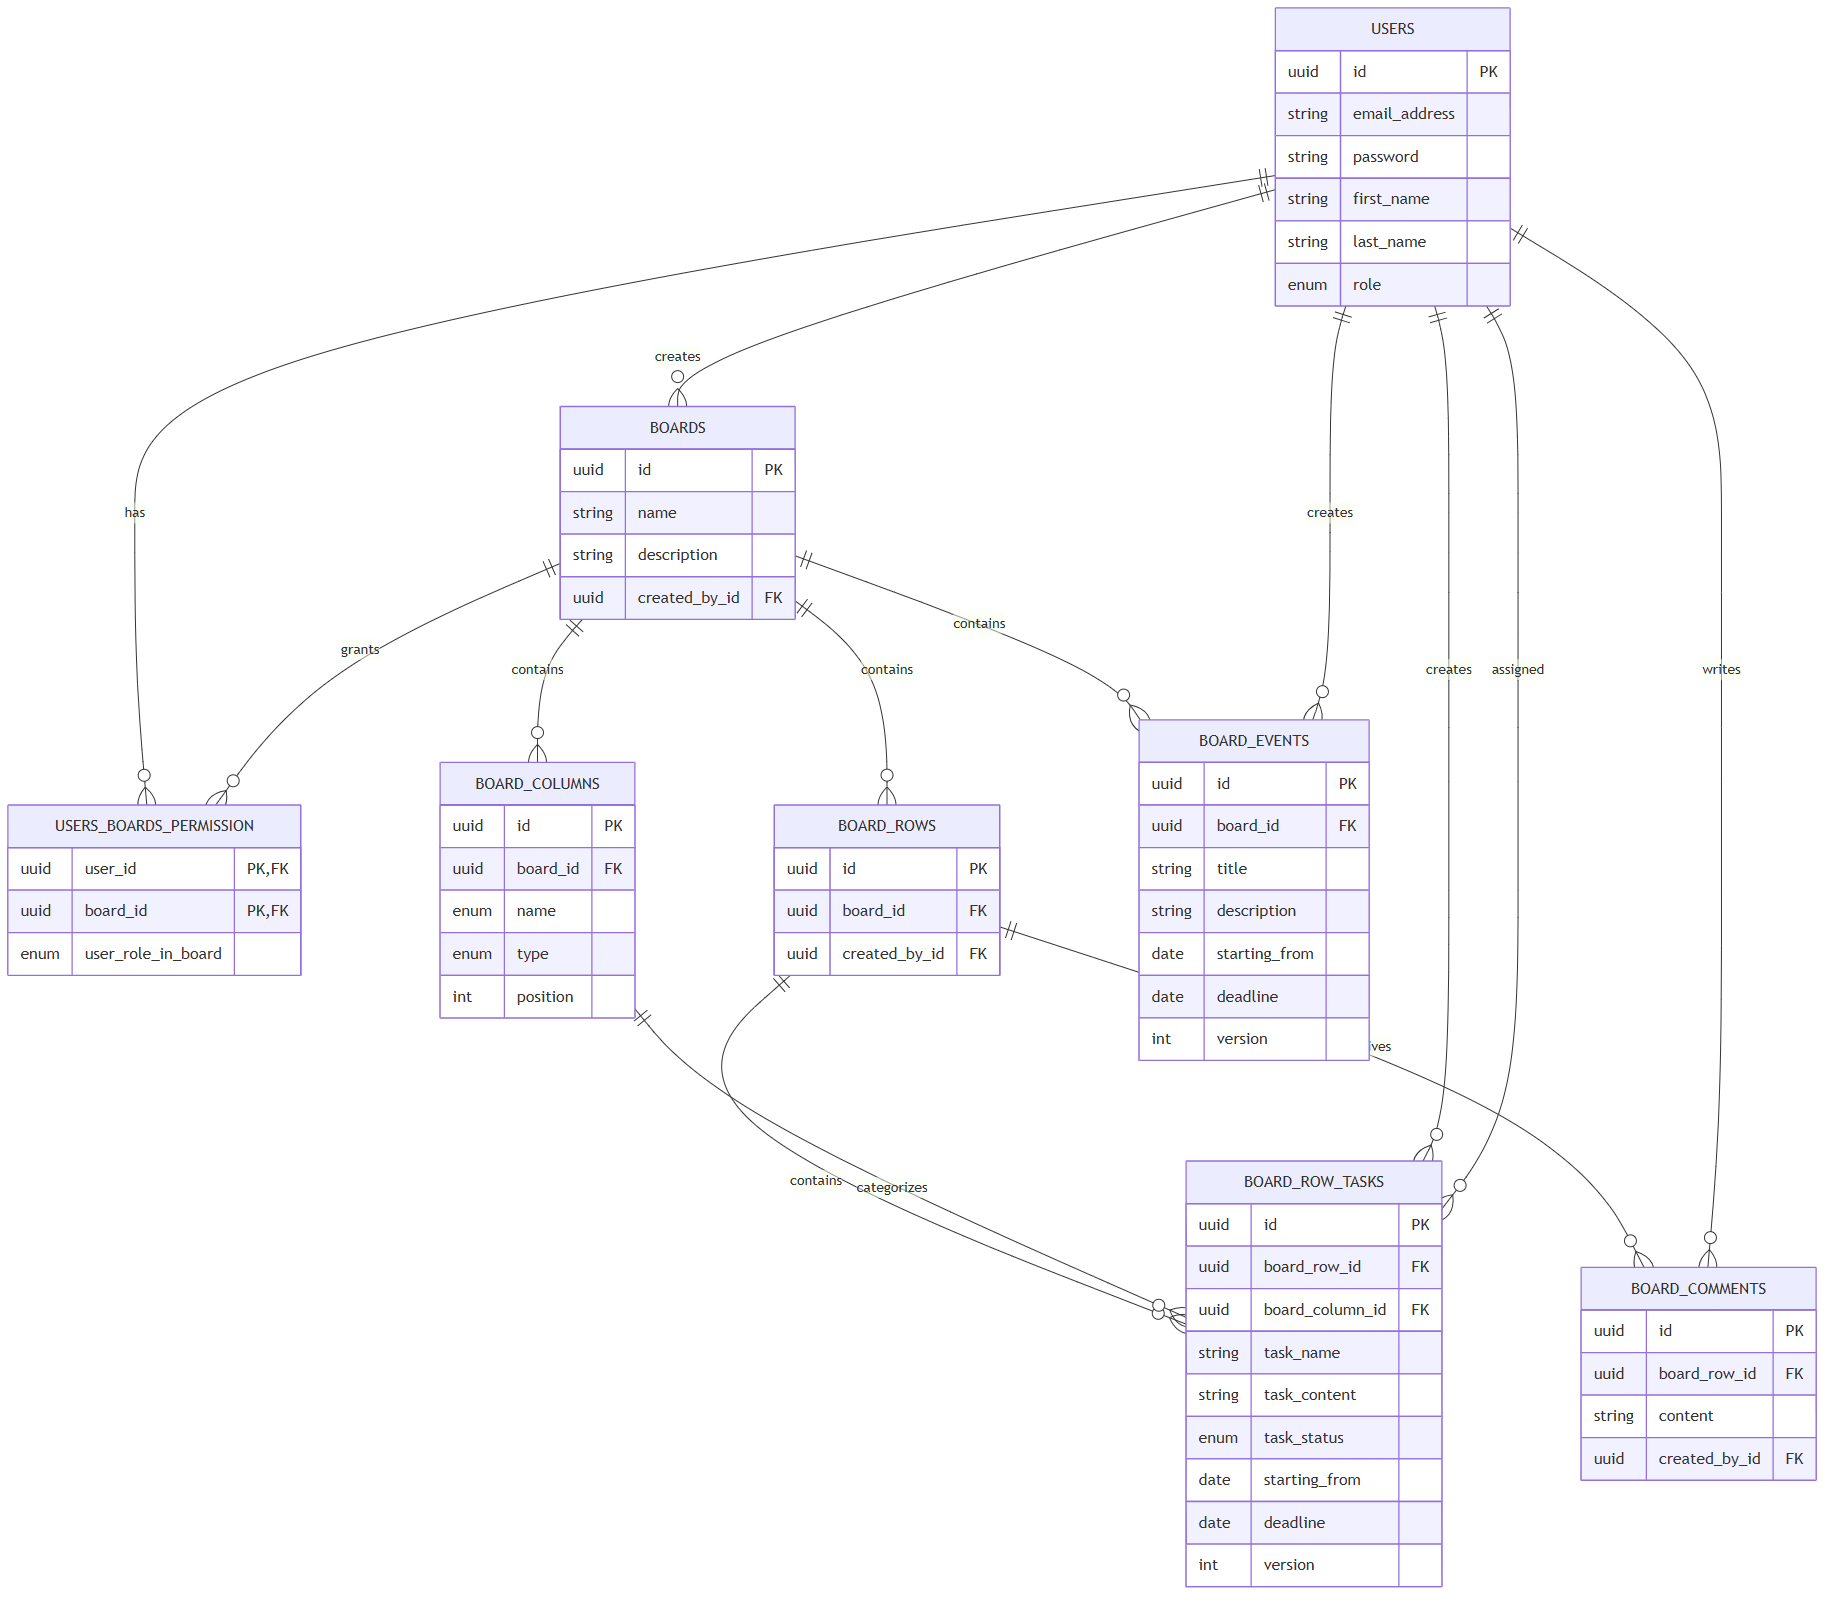
\includegraphics[width=\linewidth,height=0.78\textheight,keepaspectratio]{assets/diagrams/data_model.png}
  \caption{Modèle relationnel principal généré depuis Mermaid}
\end{figure}

\begin{longtable}{p{0.25\linewidth}p{0.65\linewidth}}
\toprule
\textbf{Table} & \textbf{Rôle} \\
\midrule
\texttt{users} & Identité applicative, email unique, mot de passe hash, prénom, nom, rôle global ADMIN ou USER. \\
\texttt{boards} & Tableau collaboratif avec nom, description, créateur et timestamps. \\
\texttt{users\_boards\_permission} & Table pivot entre utilisateur et board, avec rôle OWNER, EDITOR ou VIEWER. \\
\texttt{board\_columns} & Colonnes configurables du board : TaskID, TaskName, TaskContent, TaskStatus, Deadline, etc. \\
\texttt{board\_rows} & Ligne horizontale d'un board, support des tâches et commentaires. \\
\texttt{board\_row\_tasks} & Tâche positionnée dans une ligne et une colonne, avec statut, dates, assignation et version. \\
\texttt{board\_comments} & Commentaires sur une ligne de board. \\
\texttt{board\_events} & Événements de calendrier liés à un board, avec dates et version. \\
\bottomrule
\end{longtable}

\section{Gestion de la concurrence}

Le code implémente un verrouillage optimiste sur les tâches via le champ \texttt{version}. Lors d'une mise à jour de \texttt{BoardRowTask}, le repository exécute une mise à jour conditionnelle :

\begin{lstlisting}[caption={Principe du verrouillage optimiste}]
UPDATE board_row_tasks
SET ..., version = version + 1
WHERE id = :task_id
AND version = :version_from_client;
\end{lstlisting}

Si aucune ligne n'est modifiée, le repository retourne \texttt{None}. La couche service transforme ce résultat en exception de concurrence, puis la route renvoie une erreur HTTP adaptée. Cela évite qu'un utilisateur écrase silencieusement la modification d'un autre utilisateur.

\section{Docker et déploiement local}

Le fichier \texttt{docker-compose.yml} orchestre cinq conteneurs :

\begin{itemize}[leftmargin=*]
  \item \texttt{mysql\_db} : image \texttt{mysql:9.6.0}, port 3306, volume persistant \texttt{mysql\_data}, healthcheck \texttt{mysqladmin ping}.
  \item \texttt{database\_seed} : image \texttt{antonind5/goat-calendar-database\_service}, attend que MySQL soit sain, puis se termine.
  \item \texttt{auth\_service} : image \texttt{antonind5/goat-calendar-auth\_service}, port 5001, \texttt{FRONT\_URL=http://localhost:8080}.
  \item \texttt{board\_service} : image \texttt{antonind5/goat-calendar-board\_service}, port 5002, \texttt{FRONT\_URL=http://localhost:8080}.
  \item \texttt{front\_service} : build local depuis \texttt{production/Dockerfile.FrontService}, port 8080 vers Nginx port 80.
\end{itemize}

\begin{figure}[H]
  \centering
  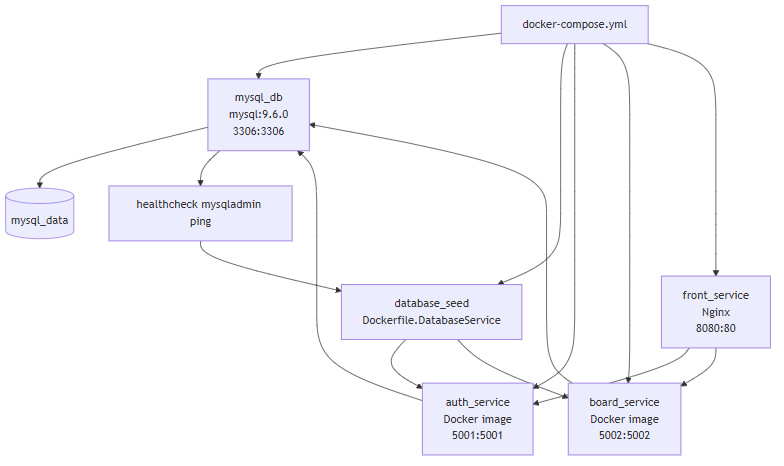
\includegraphics[width=\linewidth,height=0.72\textheight,keepaspectratio]{assets/diagrams/deployment.png}
  \caption{Déploiement Docker Compose généré depuis Mermaid}
\end{figure}

\section{Pipeline DevOps et qualité}

\subsection{Gestion des dépendances}

Chaque package Python utilise PDM avec \texttt{pyproject.toml} et \texttt{pdm.lock}. Les dépendances locales entre packages sont explicites en mode développement. Les dépendances de production sont exportées dans les Dockerfiles avec \texttt{pdm export}. Le front ne nécessite pas de build Node : il est copié tel quel dans l'image Nginx.

\subsection{Qualité statique}

Ruff est déclaré et configuré dans les packages Python. Les scripts PDM principaux sont :

\begin{itemize}[leftmargin=*]
  \item \texttt{ruff\_format} : formatage ;
  \item \texttt{ruff\_lint} : vérification et correction automatique ;
  \item \texttt{ruff\_all} : exécution combinée.
\end{itemize}

SonarCloud est configuré à la racine avec :

\begin{itemize}[leftmargin=*]
  \item organisation : \texttt{goatssoftware} ;
  \item project key : \texttt{GoatsSoftware\_GoatCalendar} ;
  \item exclusion du front dans l'analyse Sonar Python ;
  \item chemins de couverture : \texttt{coverage-reports/coverage-database\_service.xml}, \texttt{coverage-shared\_models.xml}, \texttt{coverage-auth\_service.xml}, \texttt{coverage-board\_service.xml}.
\end{itemize}

\subsection{Pipeline CI cible}

Le diagramme ci-dessous décrit la pipeline cible pour automatiser les étapes déjà préparées : installation Python 3.13, PDM, lint Ruff, tests Pytest, couverture XML, build Docker et analyse SonarCloud.

\begin{figure}[H]
  \centering
  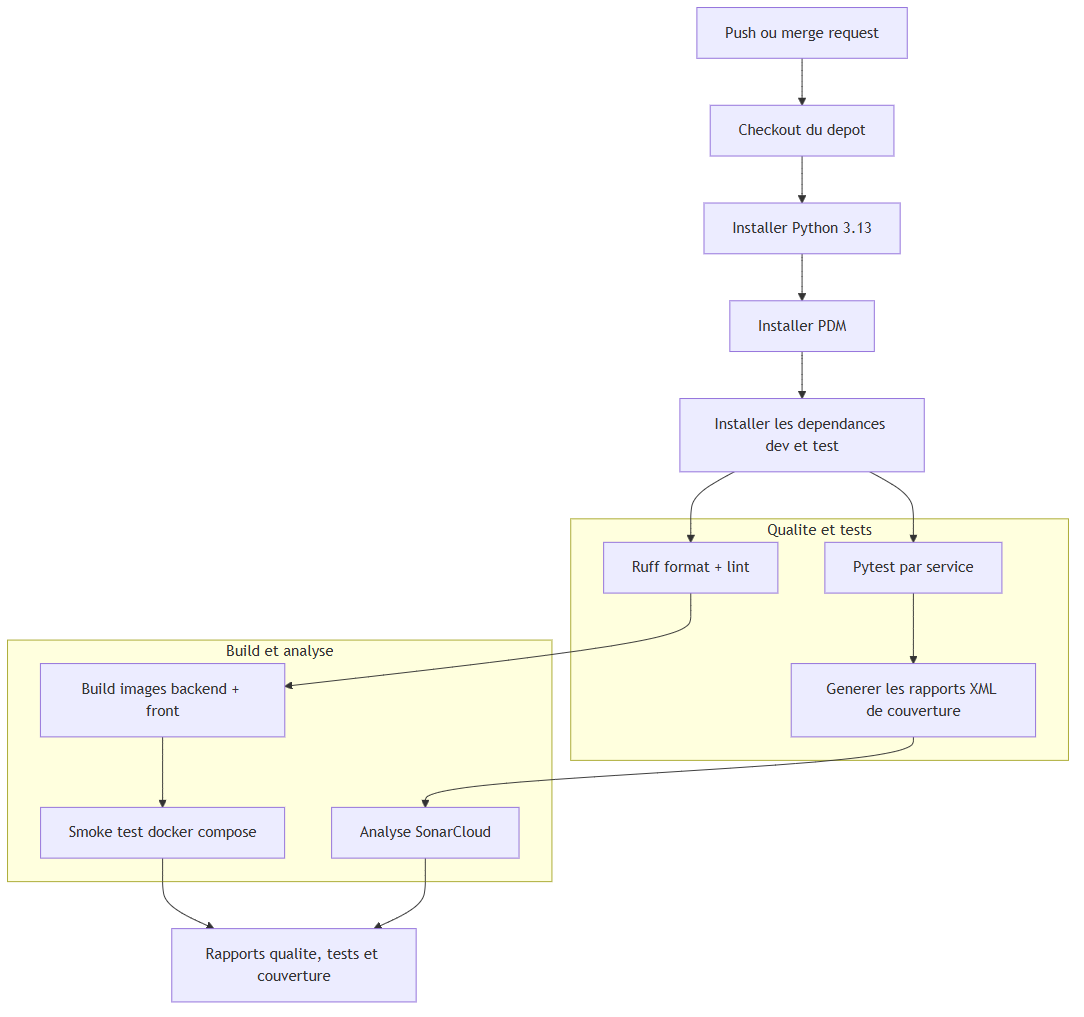
\includegraphics[width=\linewidth,height=0.62\textheight,keepaspectratio]{assets/diagrams/ci_pipeline.png}
  \caption{Pipeline CI cible générée depuis Mermaid}
\end{figure}

\subsection{Liens et résultats}

Les résultats de la qualité et de l'intégration continue sont consultables sur les plateformes suivantes :

\begin{itemize}[leftmargin=*]
  \item SonarCloud : \url{https://sonarcloud.io/project/overview?id=GoatsSoftware_GoatCalendar}
  \item GitHub Actions : \url{https://github.com/GoatsSoftware/GoatCalendar/actions}
\end{itemize}

\begin{figure}[H]
  \centering
  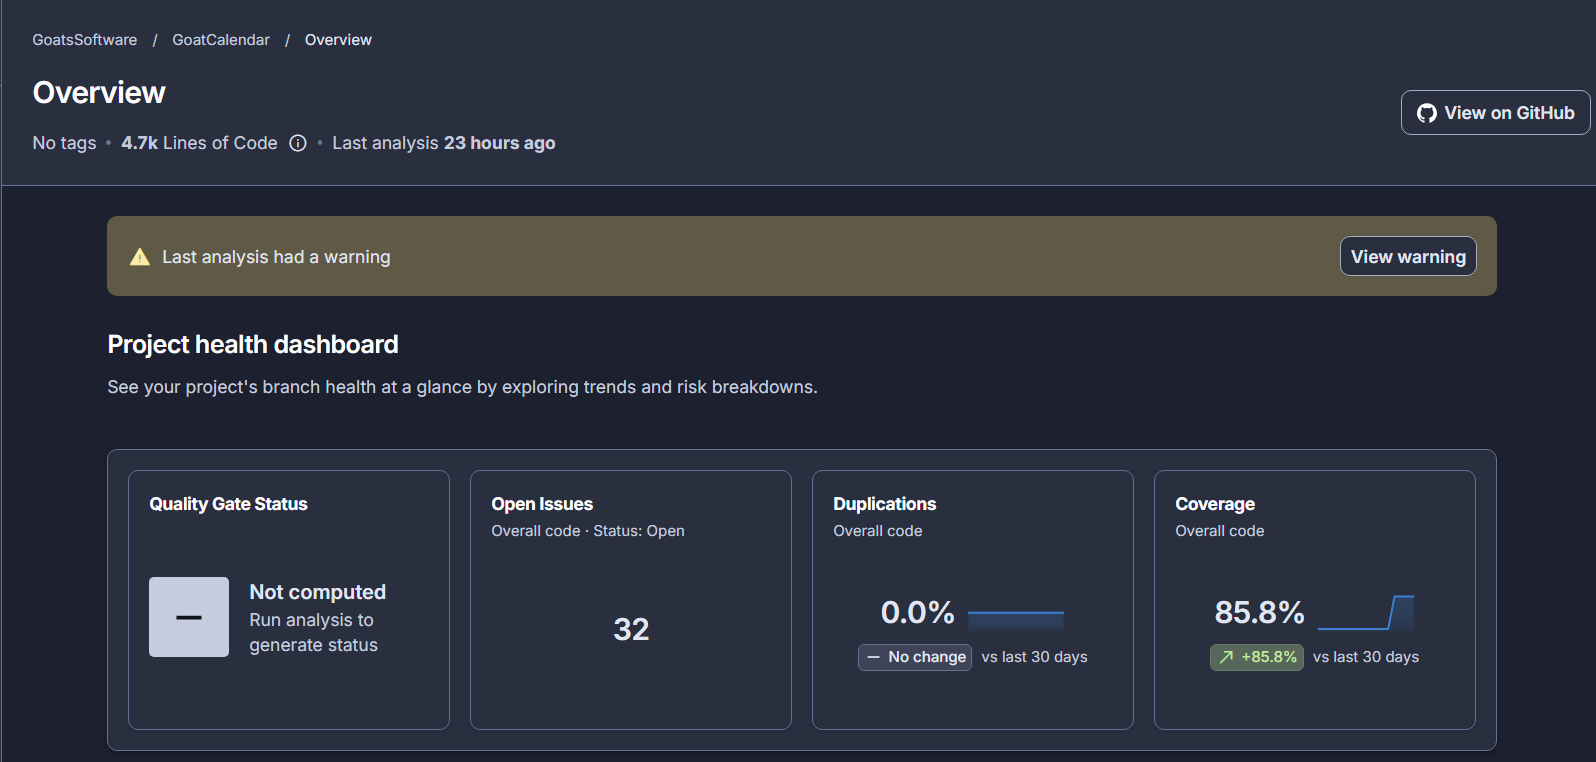
\includegraphics[width=\linewidth,height=0.72\textheight,keepaspectratio]{assets/sonarqube_page.png}
  \caption{Résultats SonarCloud du projet Goat Calendar}
\end{figure}

\begin{figure}[H]
  \centering
  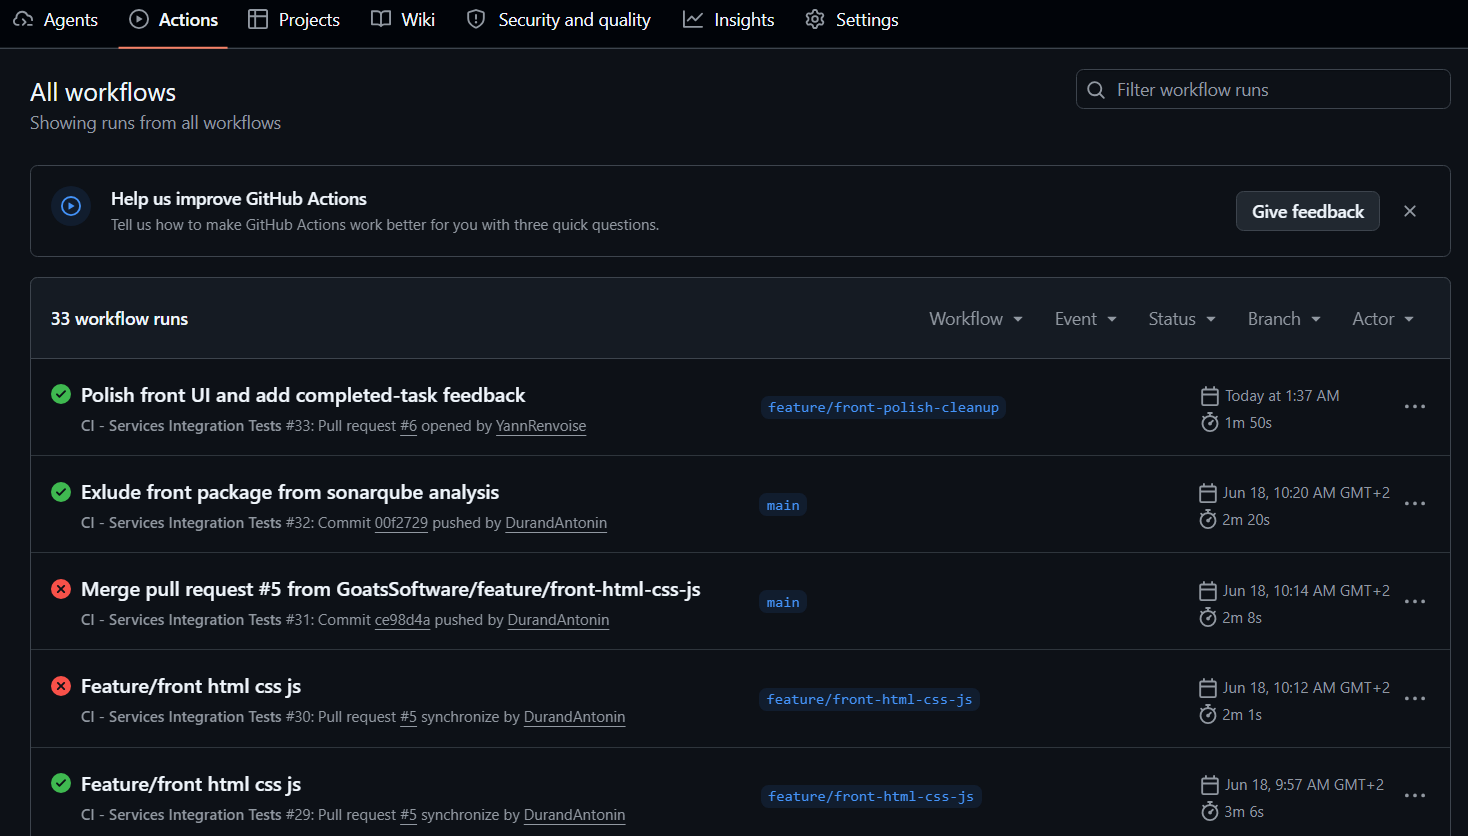
\includegraphics[width=\linewidth,height=0.72\textheight,keepaspectratio]{assets/github_action_page.png}
  \caption{Résultats GitHub Actions du projet Goat Calendar}
\end{figure}

\section{Tests et couverture}

La version finale contient 93 fonctions de test Pytest, réparties dans les quatre packages backend :

\begin{itemize}[leftmargin=*]
  \item \texttt{auth\_service/tests} : routes d'authentification, services, repository utilisateur, hash et JWT.
  \item \texttt{board\_service/tests} : services, repositories, routes boards, rows et tasks.
  \item \texttt{database\_service/tests} : database, seeder et main.
  \item \texttt{shared\_models/tests} : settings, schémas, enums et DTO.
\end{itemize}

Les dépendances de test incluent \texttt{pytest} et \texttt{pytest-cov}. Les rapports de couverture attendus par SonarCloud sont séparés par package dans \texttt{coverage-reports}.

\section{Données seed}

Le seed crée un jeu de démonstration cohérent :

\begin{itemize}[leftmargin=*]
  \item trois utilisateurs : Alice Proprio, Bob Locataire, Claire Mixte ;
  \item un board : \texttt{Demo Board} ;
  \item cinq colonnes : \texttt{TaskID}, \texttt{TaskName}, \texttt{TaskContent}, \texttt{TaskStatus}, \texttt{Deadline} ;
  \item cinq lignes ;
  \item vingt-cinq tâches, soit cinq tâches par ligne ;
  \item un commentaire par ligne ;
  \item deux événements : \texttt{Kickoff} et \texttt{Mid Review} ;
  \item deux permissions explicites : un EDITOR et un VIEWER.
\end{itemize}

Les comptes de démo utilisés par le front sont :

\begin{itemize}[leftmargin=*]
  \item \texttt{aliceproprio@gmail.com}
  \item \texttt{boblocataire@gmail.com}
  \item \texttt{clairemixte@gmail.com}
\end{itemize}

Le mot de passe de démonstration est \texttt{azerty}.

\section{Sécurité et configuration}

Les services utilisent CORS avec \texttt{FRONT\_URL}, OAuth2 Bearer token, JWT et hash Argon2. Les variables d'environnement de production sont partiellement injectées dans \texttt{docker-compose.yml}. Les identifiants MySQL et certaines clés de démonstration restent visibles dans les fichiers de configuration et le README. Pour une production réelle, ces valeurs devraient être déplacées vers des secrets Docker, des variables CI/CD ou des fichiers \texttt{.env} non versionnés.

\section{Limites actuelles}

\begin{itemize}[leftmargin=*]
  \item Le front est statique et ne contient pas de tests automatisés JavaScript.
  \item Les secrets de démonstration sont visibles dans les fichiers de configuration.
  \item Certains docstrings backend semblent provenir d'un ancien domaine métier et devraient être harmonisés avec Goat Calendar.
\end{itemize}

\section{Conclusion}

Goat Calendar présente une base DevOps complète pour le cadre du projet : architecture en couches, services backend séparés, front web bonus, base MySQL, Docker Compose, tests Pytest, qualité Ruff et configuration SonarCloud. Le projet respecte les attentes principales du sujet et ajoute les deux bonus importants : interface web et base de données.

\appendix
\section{Annexe : Google Labs}

\begin{figure}[H]
  \centering
  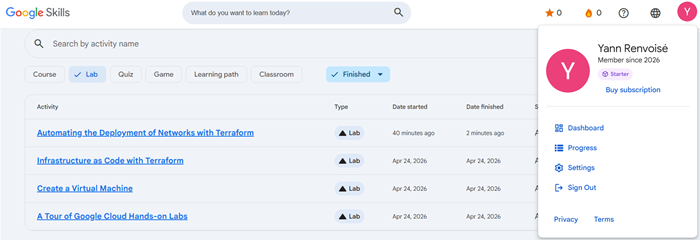
\includegraphics[width=0.95\linewidth,height=0.36\textheight,keepaspectratio]{assets/google_labs_yann.png}
  \par\smallskip
  \textbf{Yann Renvoisé}
  \par\medskip
  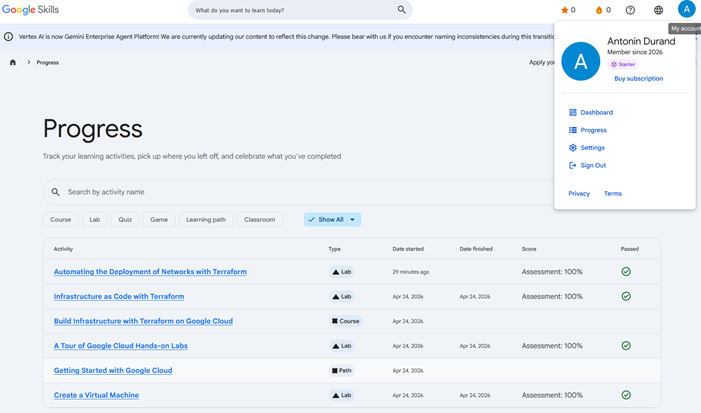
\includegraphics[width=0.95\linewidth,height=0.36\textheight,keepaspectratio]{assets/google_labs_antonin.png}
  \par\smallskip
  \textbf{Antonin Durand}
  \caption{Captures Google Labs}
\end{figure}

\section{Annexe : Sources Mermaid}

\subsection{Architecture}
\lstinputlisting[language=Mermaid]{diagrams/architecture.mmd}

\subsection{Couches}
\lstinputlisting[language=Mermaid]{diagrams/layers.mmd}

\subsection{Modèle de données}
\lstinputlisting[language=Mermaid]{diagrams/data_model.mmd}

\subsection{Déploiement}
\lstinputlisting[language=Mermaid]{diagrams/deployment.mmd}

\subsection{Pipeline}
\lstinputlisting[language=Mermaid]{diagrams/ci_pipeline.mmd}

\end{document}
